\chapter{The Web's first steps}
\label{chap_one}

\section*{Introduction}
In October 1967, a plan for a computer network, called by ARPANET (Advanced Research Projects Agency Network)\cite{history}, was presented. Three years later, the first four-computer network was up and running, making it the first step towards today's network. Later in 1982, ARPANET had officially launched the TCP/IP - the Internet, as we know it, had arrived, which finally led to the birth of the World Wide Web in the 1990s. 
\newpage


\section{Web's first generation}
\label{sec_web}
 
\subsection{History}
\label{subsec_history}
The ideas behind the World-Wide Web were formulated at CERN (European Organization for Nuclear Research) in 1989, leading to a proposal submitted in November 1990 by Tim Berners-Lee and Robert Cailliau for a “Universal hypertext system” [1]. In the four years since the original proposal, the growth of the World Wide Web had been phenomenal. It was mainly used for research applications thus, it quickly expanded until it reached people’s homes.
The World Wide Web is designed around hypertext documents that are simple in which words, phrases, or images act as links to other documents through Client-Server architecture, where the documents are stored in the server’s hard drive and can be consulted by clients from the same network through the HTTP. These documents are classified as a set of HTML pages.
In July 1994, CERN began to overturn the Web project to a new group called the W3 organization, which is now known as the W3C (World Wide Web Consortium) that was founded by Tim Berners-Lee  \cite{hist}.

In 1995, 18 million American homes were already online and Microsoft had just launched the first version of Internet Explorer, the rival of Netscape. Later that year, the first search engine “AltaVista” was introduced. It was the first and most important search engine amongst all others because it led the way for Google, the best search engine by far, to be launched in 1998. It uses automated programs called spiders like most other engines do and has a large index of keywords. It also ranks each Web page after determining their relevancy.


\subsection{Web's first technologies}

Shortly after the birth of the Web, several technologies were built. They led the way for many other languages and features to come in the next few years.  


\subsubsection{SGML}
\label{subsubsec_sgml}
The SGML (Standard Generalized Markup Language) is a standard of ISO (International Organization for Standardization) under the ISO 8879 standard. It is a standardized markup language for describing the structure and formatting of a computer document. Sections of the document are set off by embedded tags. The tags and the relationships among the groups they represent are described in a DTD (Document Type Definition). The tags do not directly specify what the display of the document will look like, so different applications can display the information differently. 

\subsubsection{DTD}
\label{subsubsec_dtd}

DTD  (Document Type Definition) is a set of markup declarations that can be used to define a document type for SGML documents. Since XML is a subset of SGML, DTD can also be used to define a document type for XML documents. If an SGML or XML document is said to be valid against a DTD document type, all elements, attributes and entities in the document must meet their declared formats described in the DTD document type. The DTD can be written inside or outside the markup language document as DTD file. Here is a simple example of a DTD document type (Listing \ref{dtdfile}), where the root element is a candidate which is defined with the sub elements: name, age, occupation and residence.\\  

\begin{lstlisting}[captionpos=b, caption=An example of a DTD file, label={dtdfile},
basicstyle=\footnotesize,frame=none]
<!ELEMENT candidate (name,age,occupation,residence)>
<!ELEMENT name (#PCDATA)>
<!ELEMENT age (#PCDATA)>
<!ELEMENT occupation (#PCDATA)>
<!ELEMENT residence (#PCDATA)>
]>     
\end{lstlisting}


\subsubsection{HTML}
\label{subsubsec_html}


HTML (Hypertext Markup Language) is a simplified derivative of SGML. It is also defined with a DTD and must meet all the markup declarations located inside the DTD in order to be valid.  Each HTML document is divided into a heading section and a main body. HTML also distinguishes headers, lists, tables, forms, etc. It is also possible to insert images or animations at specific positions in a document. 
Originally, HTML was primarily designed as a language for semantically-describing scientific documents. Its general design, however, has enabled it to be adapted over the subsequent years to describe a number of other types of documents and applications. In October 2014, HTML5 [3] was standardized by the W3C. The current version of HTML now is HTML 5.1 [4] that was recommended by the W3C in November 2016. 


\subsubsection{URL}
\label{subsubsec_url}
The final and most important keys to the World Wide Web are the URLs that allow the hypertext documents to point to other documents located anywhere on the Web. 
A URL consists of three major components: 
%%<protocol> :// <node> / <resource name> \\
\begin{lstlisting}[captionpos=b, caption=URL components, label=url, belowskip=1em, aboveskip=2em,frame=single,]
	"  <protocol> :// <node> / <resource name(path)>  "
\end{lstlisting}

 The first component specifies the protocol to be used to access the document, e.g. HTTP, FTP, etc. The second component, called the node, specifies the hostname and the file path on the network from which the document is to be obtained, and the third component specifies the location of the document on the remote machine.


\subsection{Limitations of the first generation of the Web}

The Web is limited to the use of static HTML documents, the lack of context and the absence of human interaction. This led to move to a new generation of the Web.  

% Une section
\section{Web's second version}
\label{sec_web2_0}

% Une sous section
\subsection{Preface}
\label{subsec_pres_web_2_0}

The second generation of the Web \cite{web2030} had introduced  to a diversity of new applications and services of the Web such as social networking (Facebook, Twitter, ...), blogging, wikis, photo and video sharing (Youtube, Flickr, ...), tagging, etc. What these new applications had in common was that the user had become the source of information on the Web. These new dynamic Web apps are distinguished by some features : 

 \begin{itemize}
 \item \textbf{Folksonomy:} It's the free classification of information on the World Wide Web known as social tagging.
 \item \textbf{Rich User Experience:} The social Web uses new technologies presenting dynamic and rich user experience to users. %%Unlike the first generation of the Web  ;
 \item \textbf{User As Contributor :} The user is able to contribute to the content by means of Evaluation, Review and Commenting, etc.
 \end{itemize}
		
\subsection{New technologies and Languages}
\label{subsec_app_tech}
\subsubsection{XML}
XML (Extensible Markup Language) is a formal recommendation from the W3C \cite{xml}, and is similar to HTML for containing markup symbols. An XML document contains elements defined by tags. An element has a beginning and an ending tag. All elements in an XML document are contained in an outermost element known as the root element. This allows XML to support hierarchical structures.  

In order for an XML document to be valid, all elements, attributes and entities in the document must meet their declared formats described in the DTD document type.\\
The listing \ref{dtdfile} above shows the DTD related to the XML document shown in the listing \ref{xmlfile} below.

\begin{lstlisting}[captionpos=b, caption=An example of an XML file, label={xmlfile},
basicstyle=\footnotesize,frame=none]
<?xml version="1.0"?>
<candidate>
  <name> Francois Fillon </name >
  <age> 63 </age >
  <occupation> French politician </occupation >
  <residence> Le Mans </residence >
</candidate>
\end{lstlisting}

\subsubsection{XML Schema}
Similar to DTD, XML Schema \cite{xmlshema} is also a language for expressing constraints about XML documents. It is usually named XML Schema Definition or simply XSD file. Unlike DTD documents, XML Schema uses an XML-based syntax, whereas DTDs have a unique syntax. It defines datatypes for elements and attributes while DTDs do not. It also defines the number and order of child elements, while DTDs do not. And most importantly XML schema is extensible, while DTDs are not.\\
The listing \ref{xmlfshema} below, shows the content of an XSD file that defines and describes the XML document shown in the listing above \ref{xmlfile}. 

\begin{lstlisting}[captionpos=b, caption=An example of a XML Schema file, label={xmlfshema},
basicstyle=\footnotesize,frame=none]
<?xml version="1.0"?>
<xs:schema xmlns:xs="http://www.w3.org/2001/XMLSchema">
  <xs:element name="Candidate">
    <xs:complexType>
      <xs:sequence>
        <xs:element type="xs:string" name="name"/>
        <xs:element type="xs:string" name="age"/>
        <xs:element type="xs:string" name="occupation"/>
        <xs:element type="xs:string" name="residence"/>
      </xs:sequence>
    </xs:complexType>
  </xs:element>
</xs:schema>

\end{lstlisting}

\subsubsection{RSS}

RSS (Really Simple Syndication) \cite{rss} is a Web service that has a main focus of facilitation of browsing for news and updates related to a certain website. The RSS feed is an XML document that is usually used by news, companies' sites, or blogs in order to quickly represent their latest information (e.g. headlines, articles,events, etc.) automatically. RSS feed can be gathered and sorted using a software called RSS Aggregator that checks automatically for new content and immediately converts this new content to a readable format. Browsing websites can be very time-consuming especially with low bandwidth. Thus, with the use of RSS feed, users could save plenty of time.

\subsubsection{DOM}

DOM (DocumentObjectModel) is a neutral interface that allows languages and scripts to have a dynamic access and update of the content, structure and style of XML and HTML documents\cite{dom}. \\
The first level of DOM, published in 1998, is separated in two parts: the HTML and Core. The document is presented as a tree of document's elements like paragraphs, buttons, and list. It allow to parse, add, delete, and modify its elements.  \\ 
The DOM level 2, published in 2000, is build on DOM level 1 and has 6 parts: Core, HTML, Events, Style, View and Traversal and Range. It allows immediately to identify an element or group of elements in a document. Also, it offers a direct access to a particular element in the document using the function getElementById() \cite{dom2}.\\
The Dom level 3, published in 2004, comes with XPath module, keyboard events module and XML documents serialisation interface.\\
The DOM level 4 is currently in development. The Last Call Working Draft was in February 2004. 


\subsubsection{CSS}

CSS (Cascading Style Sheets) is a language that describes the style of an HTML document including the colors, borders, backgrounds ... \\
Using HTML, we can define the structure and the style of a Web page however, the presentation is limited \cite{css} , so it is recommended to separate the structure from the style to ease the maintenance of sites.\\
A CSS rule-set consist of a selector and a declaration block:\\
The selector points to the HTML tags to style.\\ 
The declaration block is surrounded by curly braces and contains declarations of rules separated by semicolons.\\
Each declaration includes a CSS property name and a value, separated by a colon \cite{css2}.\\
In the following example, all <h2> elements will be center-aligned, with a blue text color:

{\tt \small
\centering
\begin{verbatim}
 h2 {
    color: blue;
    text-align: center;
}
\end{verbatim}
}




\subsection{Other Web Technologies}

Many languages and technologies have been introduced to make Web more interactive but they are not W3C recommendations.

\subsubsection{JavaScript}

JavaScript is an oriented object and scripts programming language that specify the behavior of Web pages making it more dynamic and interactive with the user.\\
JavaScript is a client-side language, that means that the script is executed by the browser in the user side. In fact, the browser execute the code embed within <script> HTML tag.


\subsubsection{AJAX}

AJAX (Asynchronous JavaScript And XML) aims to optimise the interactivity and the use of Web applications. AJAX allows Web pages to be updated asynchronously by exchanging data with a Web server behind the scenes. This means that it is possible to update parts of a Web page without reloading the whole page \cite{ajax}.
AJAX is the combination of many languages and technologies as presented in figure \ref{fig_Ajax} :
\begin{itemize}
    \item HTML and CSS to represent the Web page.
     \item DOM to describe the interface and display or use the data.
     \item XMLHTTPRequest to request data from a Web server.
     \item XML to structure recovered files from the server.
     \item JavaScript to exploit the XMLHTTPRequest and DOM.
\end{itemize} 
 %%\newpage 

\begin{figure}[H]
\centering
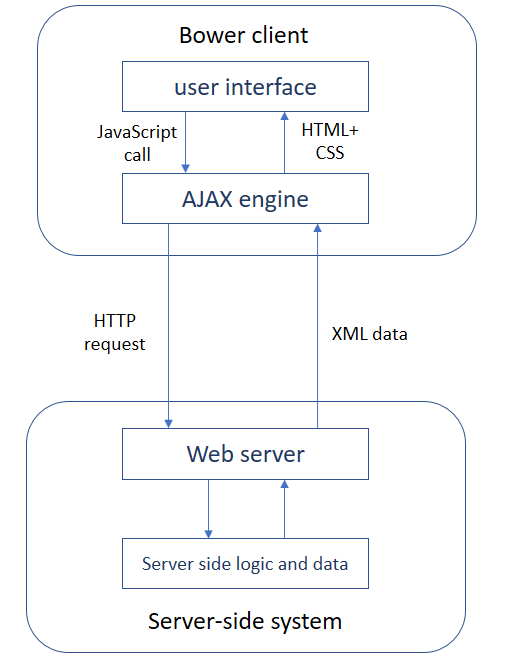
\includegraphics[scale=0.4]{ajax}
\caption{AJAX architecture }
\label{fig_Ajax}
\end{figure}


\subsection{Limitations of social Web }

Although new technologies have evolved within the second generation of the Web, a number of limitations can be identified:

\begin{itemize}
    \item Time and cost consuming: Big projects of social Web application generally take a lot of time to accomplish. 
    \item Short life of information: Once an information on the Internet gets updated, we simply cannot keep track of it so it loses its relevance gradually.  
    \item Lack of semantics: Web applications are still using legacy databases (e.g: Relation databases) without generating and representing knowledge bases.
\end{itemize}


\section{Information search in Web}

\subsection{Search engines}

A search engine is a program that returns a list of Web documents where specific keywords in the query were found \cite{search}.\\
A search engine is a database that is permanently updated by Robots or Spiders that fetch the Web pages, save their contents, and index automatically. There are many popular search engines, e.g. Google, Bing, Yahoo, Ask, etc.


\subsection{Anatomy of search engines}
To provide a pertinent search in the Web, the search engine must have 3 essential parts:
\begin{itemize}
    \item The robot (also known as Spider or Crawler).
    \item The store or the database, that includes the indexer, indexes and complex search algorithms.
    \item The Query or search Interface.
\end{itemize}

The architecture of search engines is shown in the next figure \ref{fig_search_engine}:

\begin{figure}[H]
\centering
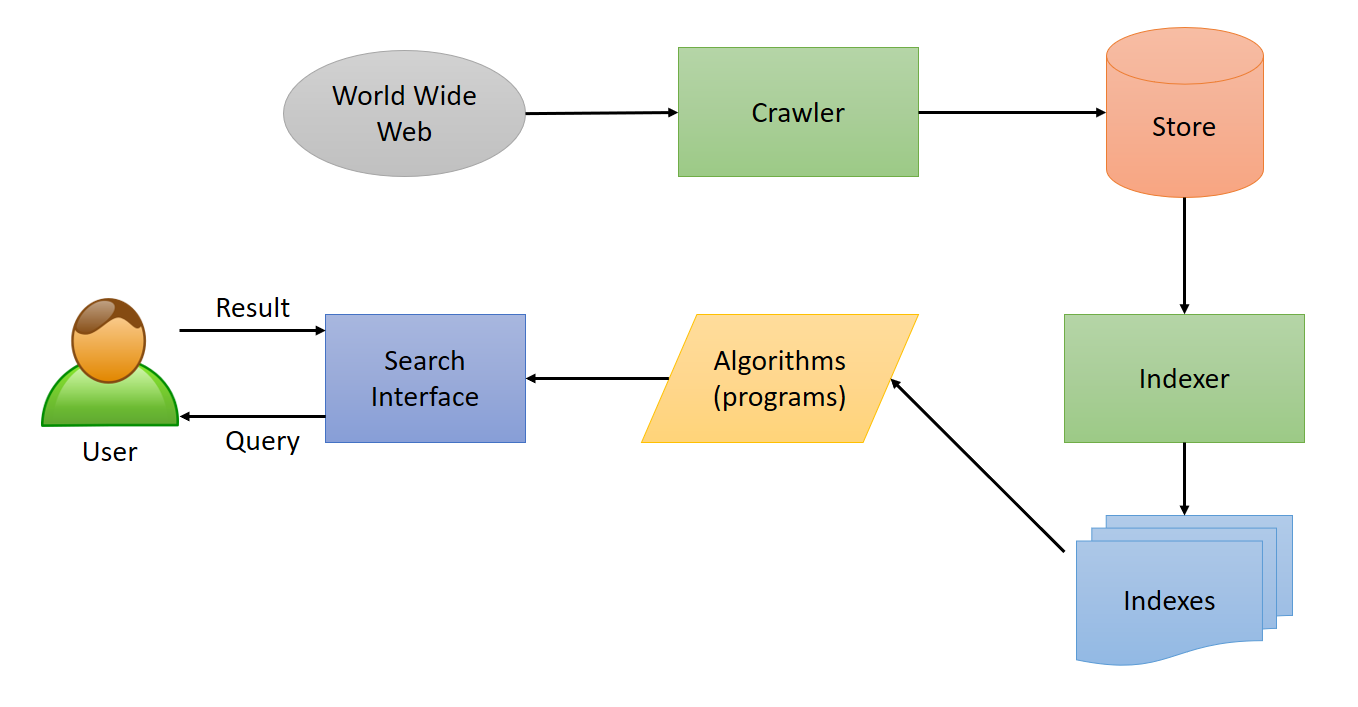
\includegraphics[scale=0.4]{searchengine}
\caption{Search engines architecture }
\label{fig_search_engine}
\end{figure}

\subsubsection{Robot}
Also called Spider or Web-crawler, the robot is the most essential part in the search engine. It collects information from Web documents to be indexed in the database. A Spider can begin almost anywhere because most Web page contains links of other pages. As soon as it sees a link to another page, it goes off and fetches it. \\Alta Vista is an example of a search engine who has many spiders working in parallel\cite{spider}.
\subsubsection{Index}
The Index is where parsed Web pages by the Spider are saved. It contains URLs and the page's title and keywords. When the Robot parse Web pages, it automatically updates the index.\\
There are many ways to index a Web page that distinguishes a search engine from another by results of a keyword query. When the robot fetches the Web pages, it uses different methods to index its content, among the best known:\begin{itemize}
    \item Full-text indexation.
    \item Manual indexation the uses a file edited by person who wants the presence of their Web pages in the database of the search engine. 
    \item Indexation by specific HTML tags (Meta,Title...).
    \item Static indexation which saves the scoring of words in the database.
\end{itemize}
\subsubsection{Query Interface}
The Query interface allows to the user to enter his query using keywords which will then be searched in the index.\\
The interface chooses among the Web pages in the index which satisfy the query and sort them in descending order of relevance, then the user can access to them using a hypertext link. 


\newpage %% a changer si nécessaire 
\section*{Conclusion}

The Web's main purpose was to be designed as a tool to share information across the world. It started with the basics of sharing a document, but has gone on to create tools that are currently known as Web applications, these tools allow us to improve and share our lives (social Web) and much more. The Web is constantly changing and evolving and it will be superseded by something even greater, faster and better. Notably, up on explosion of information amount accessible through the Web, the past versions have encountered drawbacks such as:

%%Today’s World Wide Web has achieved a great evolution. It is widely used all around the world. The simple foundations, on which it is based, has given its strength and global community. Almost every user is able to create and publish hypertext resources in a simple manner. Notably, up on explosion of information amount accessible through the Web, the past versions have encountered drawbacks. The huge amount of content required to be processed in order to find desired facts such as: 

\begin{itemize}
    \setlength{\itemsep}{0cm}
    \setlength{\parskip}{0cm}

    \item Difficulties in finding correct information through simple searching and browsing mechanisms,
    \item Problems of finding facts, which has common correspondents,
    \item Irrelevant results after providing more complex queries in the browsing engines,
    \item Lack of semantics,
    \item Lack of deduction facilities.
\end{itemize}




%Pour faire appel à cette of figure, il suffit d'utiliser le label comme suit:

%La figure \ref{fig_logo_utm} présente le logo de l'UTM.

%On peut ajouter un tableau en utilisant le syntaxe suivant:

%%Le tableau \ref{tab_val} présente ...
%%\begin{table}[htpb]
%%\centering
%%\caption{Table des valeurs ...}
%%\begin{tabular}{|c|c|c|}
%%\hline 
%%1 & 2 & 3 \\ 
%%\hline 
%%6 & 5 & 4 \\ 
%%\hline 
%%7 & 9 & 10 \\ 
%%\hline 
%%\end{tabular} 
%%\label{tab_val}
%%\end{table}